% !TeX spellcheck = en_GB 
\section{Conclusion}

interlocking can achieve 85\% of the strength of the PP and TPLA base materials; we reach about 65\%

diagonal design outperforms dovetail interlocking?

genus interlocking shows potential for high compliance materials

genus interlocking can help with complex and slanted surfaces 


\subsection{Applications}
exxplain: PP for living hinges; TPLA for stiffness


photo's of gripper, container, prosthetic hand 



\begin{figure}
	\centering
	\begin{subfigure}[B]{.33\columnwidth}
		\centering
		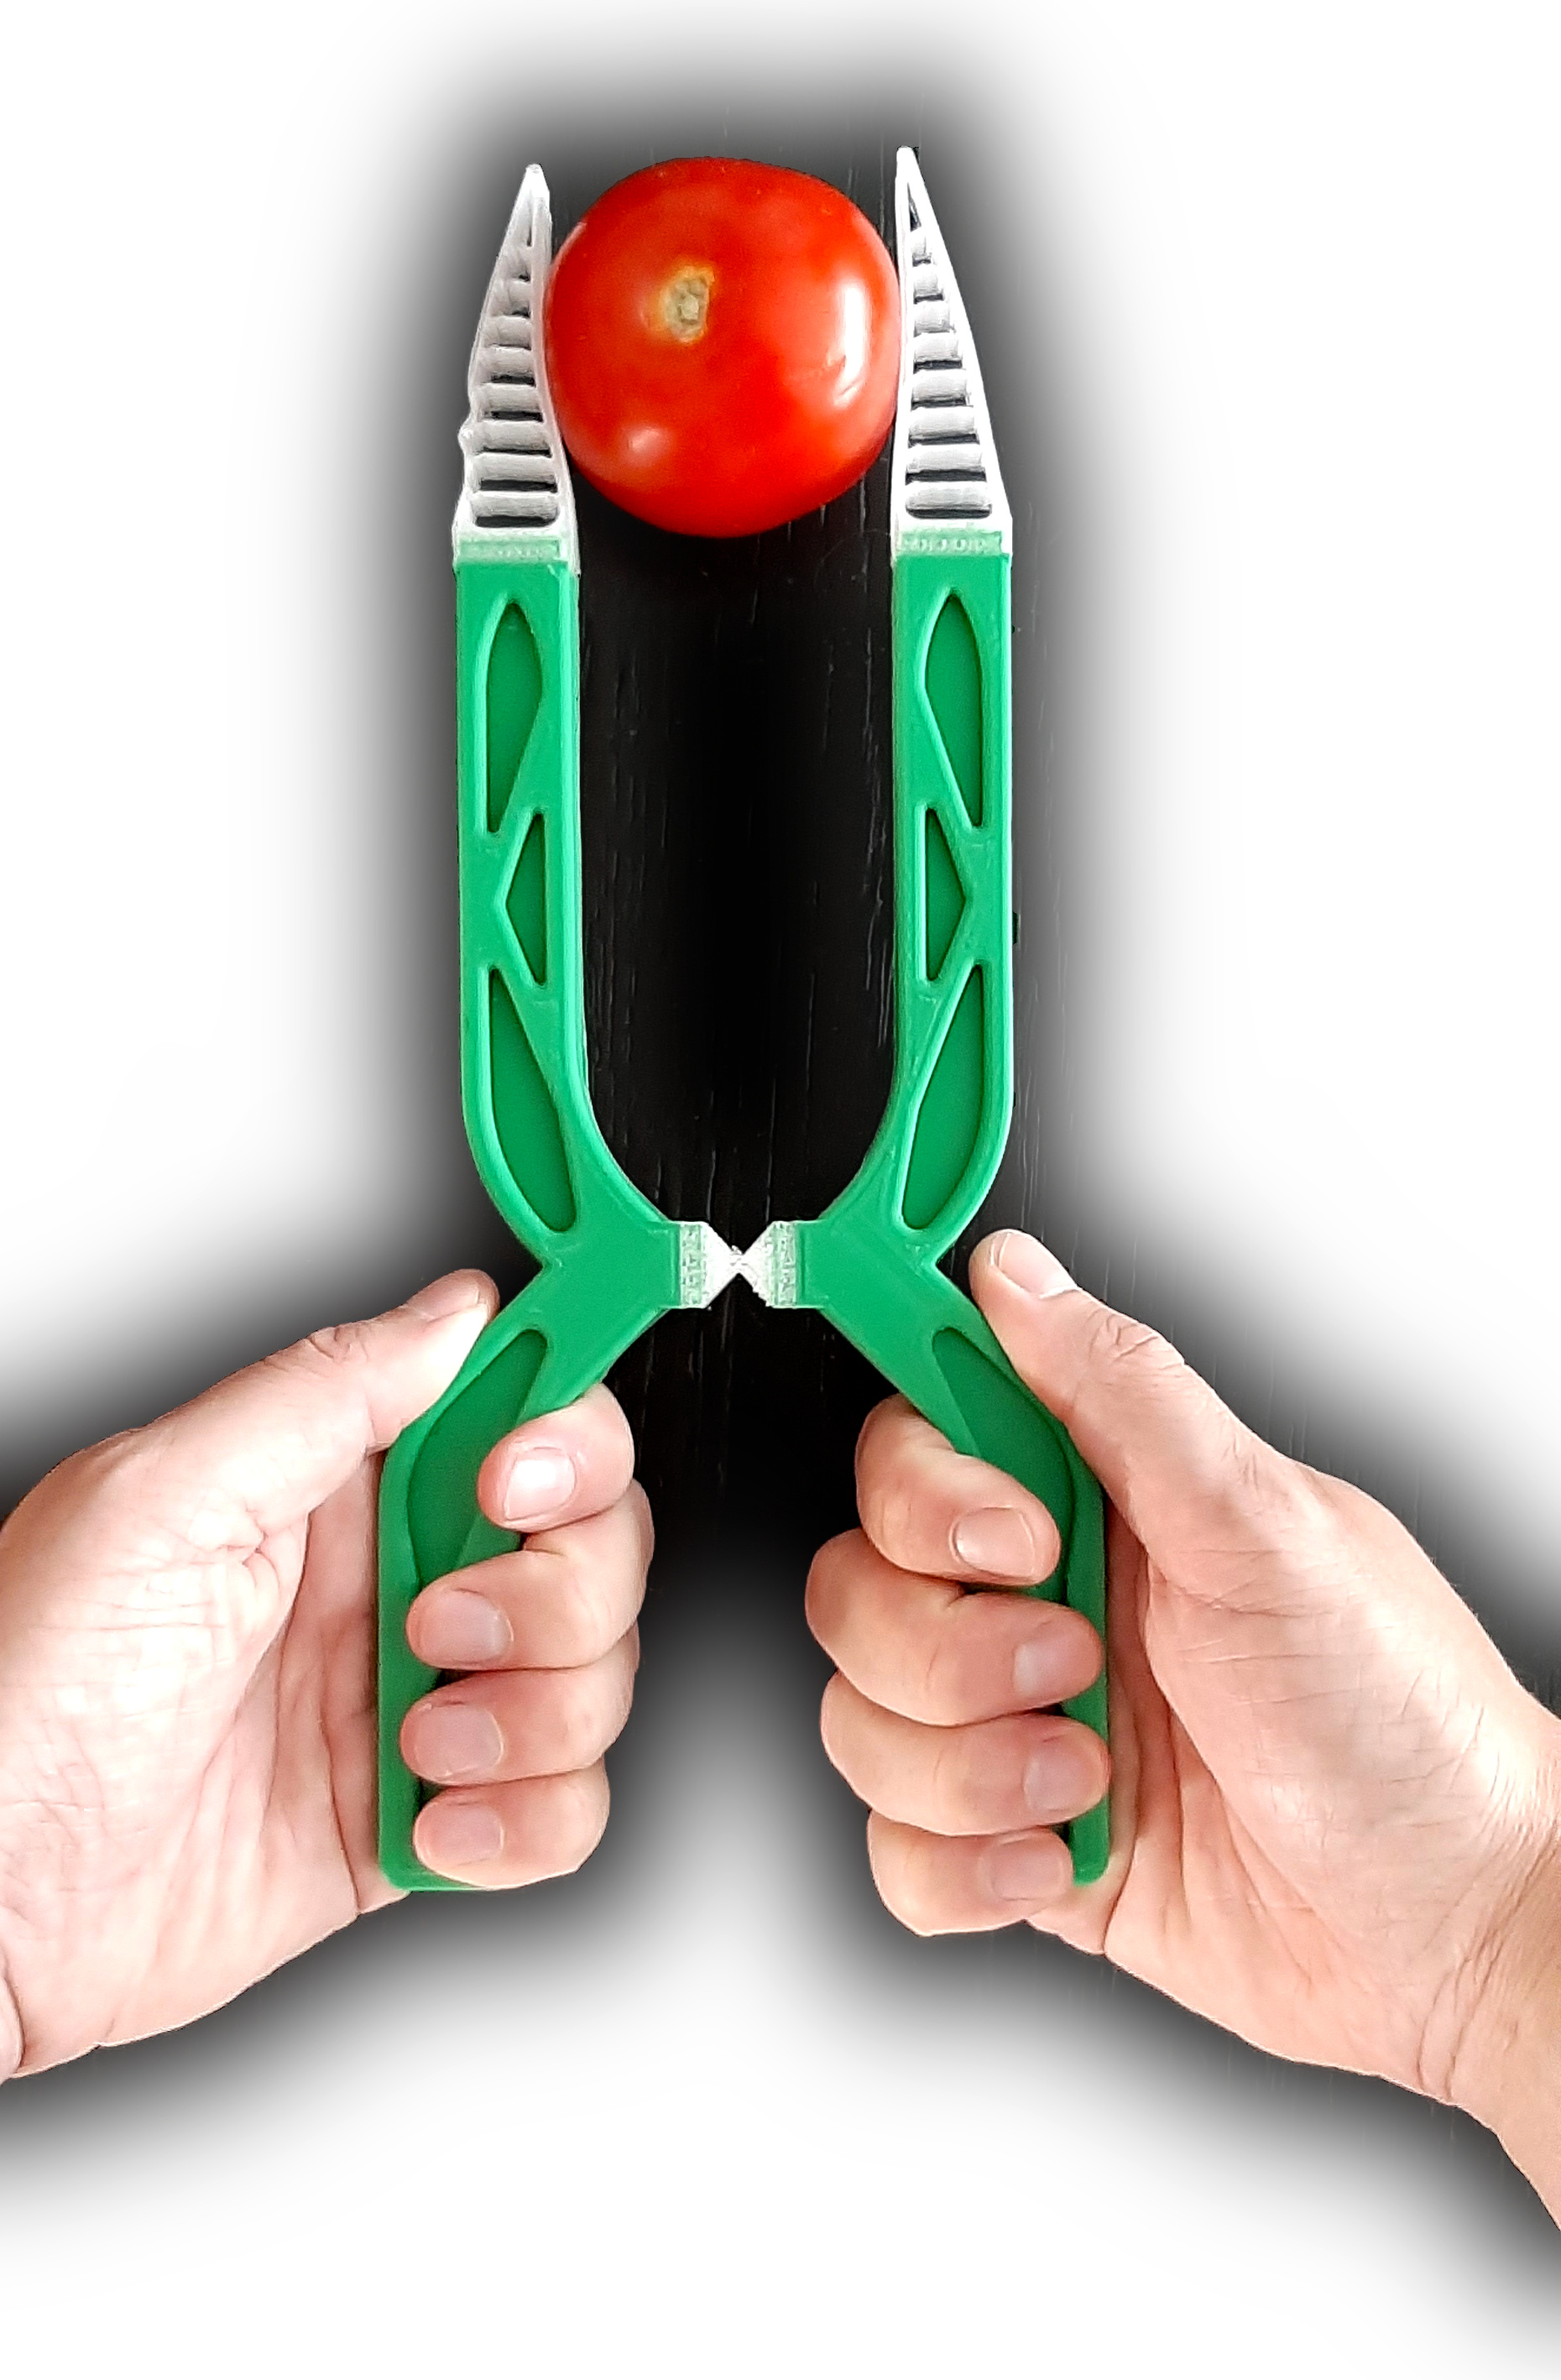
\includegraphics[width=\columnwidth]{sources/applications/gripper.jpg}
		\caption{Gripper design}
		\label{fig:gripper}
	\end{subfigure}
	\caption{Applications of interlocking structures.}
\end{figure}

optimize for complex surfaces and complex loading situations



investigate 